%%% Local Variables:
%%% TeX-command-extra-options: "-shell-escape"
%%% mode: latex
%%% TeX-master: t
%%% End:
\documentclass{beamer}
\usepackage{caption}
\usepackage{minted}
\usepackage{tikz}
\usepackage{xcolor}
\usetikzlibrary{shapes.geometric, arrows}
\tikzstyle{startstop} = [rectangle, rounded corners, minimum width=3cm, minimum height=1cm,text centered, draw=black, fill=red!30]
\tikzstyle{io} = [trapezium, trapezium left angle=70, trapezium right angle=110, minimum width=1.5cm, minimum height=0.6cm, text centered, draw=black, fill=blue!30]
\tikzstyle{process} = [rectangle, minimum width=1.5cm, minimum height=0.5cm, text centered, draw=black, fill=orange!30]
\tikzstyle{decision} = [circle, radius=2.5cm, text centered, draw=black, fill=green!30]
\tikzstyle{arrow} = [thick,->,>=stealth]
\usepackage[labelformat=simple]{subcaption}

\usetheme{Singapore}
\title{Arbitrarily Large Data}
\begin{document}
\begin{frame}
\titlepage
\end{frame}
\section{Lists}

\begin{frame}
  \huge \emph{Recursion} - see recursion
\end{frame}

\begin{frame}
  \frametitle{Self Referentiality Powerful and Scary}
  \begin{figure}
    \begin{subfigure}{0.3\textwidth}
      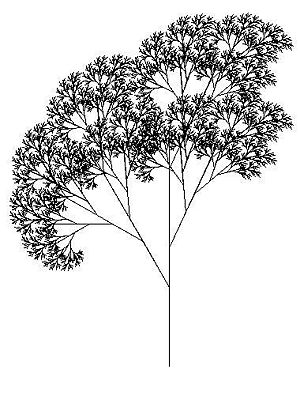
\includegraphics[width=0.9\textwidth]{images/recursive-tree.JPG}
    \end{subfigure}
    \begin{subfigure}{0.3\textwidth}
      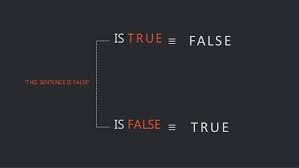
\includegraphics[width=0.9\textwidth]{images/liars-paradox.jpeg}
    \end{subfigure}
    \begin{subfigure}{0.3\textwidth}
      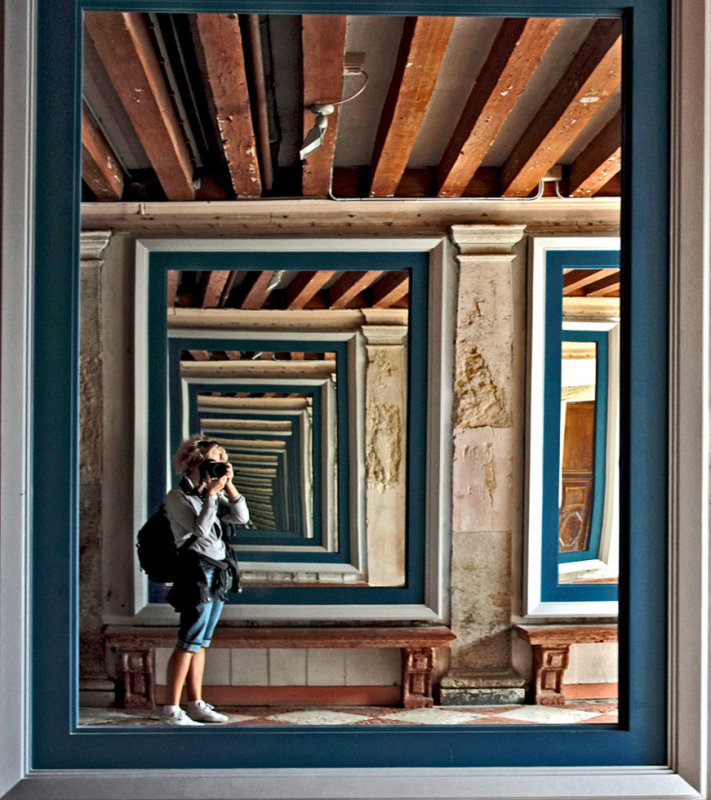
\includegraphics[width=0.9\textwidth]{images/reflections.jpg}
    \end{subfigure}
  \end{figure}
\end{frame}

\begin{frame}
  \frametitle{Self Referentiality}
  The ability to self reference is \emph{powerful} but also \emph{troublesome}.
  \begin{itemize}
  \item<2-> Through self referentiality, we can construct the most basic mathematical tool that has
    been proven to be a powerful concept throughout history--the natural numbers.
  \item<3-> This leads to many other powerful structures like other numbers, lists, trees, etc.
  \item<4-> But we also got the first instances of extremely troublesome concepts--paradoxes.
  \item<5-> The omnipotence paradox - asked if it was possible for a being to exist so powerful that it could create a stone that it could not lift.
  \item<6-> The Epimenides paradox, 'All Cretans are liars' when uttered by an ancient Greek Cretan was one of the first recorded versions. 
  \end{itemize}
\end{frame}

\begin{frame}
  \frametitle{Self Referential Data and Racket}
  So far, we have only written programs with fixed size data (well numbers and strings aren't truly fixed size but they are primitive).
  \begin{itemize}
  \item<2-> We don't currently have a way to specify data definitions for extensible data.
  \item<3-> Consequently, we can't support the creation of programs like a space invaders game with
    flexible numbers of enemies.
  \item<4-> So we will change how we specify data definitions to support things like this and will revise our design recipes
    for dealing with extensible data
  \end{itemize}
\end{frame}

\begin{frame}
  \frametitle{Lists: A Fundamental Structure }
  One of the most important things to get used to in functional programming is dealing with lists.
  
\end{frame}
\end{document}
%%% Local Variables:
%%% TeX-command-extra-options: "-shell-escape"
%%% mode: latex
%%% TeX-master: t
%%% End:
